\mysection{Hierarchical Attention}

\vspace{2\baselineskip}


    \begin{minipage}[c]{0.3\textwidth}
        \centering
        \begin{subfigure}[b]{1.\textwidth}
            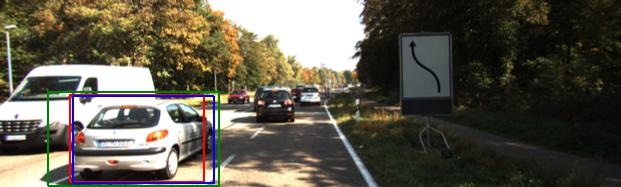
\includegraphics[width=\textwidth]{att_img}
        \end{subfigure}
        
        \hspace{-30pt}
        \begin{minipage}{.85\textwidth}
            \vspace{.5em}
            \begin{subfigure}[b]{.29\textwidth}
                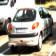
\includegraphics[width=\textwidth, cfbox=darkgreen 4pt 0pt]{att_glimpse}
            \end{subfigure}
            \hfill
            \hspace{8pt}
            \begin{subfigure}[b]{.29\textwidth}
                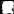
\includegraphics[width=\textwidth]{att_mask}
            \end{subfigure}
            \hfill
            \hspace{5pt}
            \begin{subfigure}[b]{.29\textwidth}
                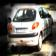
\includegraphics[width=\textwidth]{att_overlay}
            \end{subfigure}
            
        \end{minipage}
    \end{minipage}\hfill
 
    \begin{minipage}[c]{0.3\textwidth}
        \vspace{1em}
            \textcolor{blue}{Ground-truth} and \textcolor{red}{predicted} bounding boxes and an \textcolor{darkgreen}{attention glimpse}. The bottom row shows the three layers of attention: 
            \begin{description}%[labelsep=1em, leftmargin=!,labelwidth=\widthof{\bfseries Interpretable:}]
                \item [$1^{st}$]  layer extracts an attention glimpse (left)
                \item [$2^{nd}$]  layer uses appearance attention to build a location map (middle)
                \item [$3^{rd}$]  layer uses the location map to suppress distractors (right)
            \end{description}
    \end{minipage}